% В тексте следует применять научно-технические термины, обозначения
% и определения, установленные действующими стандартами, а при их
% отсутствии – принятые в научно-технической литературе.
% Запрещается применять иностранные термины при наличии
% равнозначных слов и терминов в русском языке.

% https://tex.stackexchange.com/questions/498098/how-to-fix-xelatex-warnings-about-undefined-font-shapes
% !TeX spellcheck = russian-aot-ieyo

% Зачем: Определяет класс документа (То, как будет выглядеть документ)
% Примечание: параметр draft помечает строки, вышедшие за границы страницы, прямоугольником, в финальной версии его нужно удалить.
% \documentclass[a4paper,14pt,russian,oneside,final,draft]{extreport}
\documentclass[a4paper,14pt,russian,oneside,final]{extreport}

\usepackage{float}
%\restylefloat{table}

% Зачем: чтобы выключать перенос слов (например в таблицах)
\usepackage{hyphenat}

% Зачем: Учет особенностей различных языков.
\usepackage[english,russian]{babel}

% Зачем: что-то чтобы док получился лучше, используем новую кодировку для всяких символов
\usepackage[T2A]{fontenc} 
\usepackage{fontspec}
\setmainfont{Times New Roman} % Set Times New Roman as main font
\setmonofont{Consolas}

% Зачем: Делает результирующий PDF "searchable and copyable".
\usepackage{cmap}

% Зачем: Чтобы можно было использовать русские буквы в формулах, но в случае использования предупреждать об этом.
\usepackage[warn]{mathtext}


% Зачем: Добавляет поддержу дополнительных размеров текста 8pt, 9pt, 10pt, 11pt, 12pt, 14pt, 17pt, and 20pt.
% Почему: Пункт 2.1.1 Требований по оформлению пояснительной записки.
\usepackage{extsizes}


% Зачем: Длинна, пимерно соответвующая 5 символам
% Почему: Требования содержат странное требование про отсупы в 5 символов (для немоноширинного шрифта :| )
\newlength{\fivecharsapprox}
\setlength{\fivecharsapprox}{6ex}

\usepackage{placeins}


% Зачем: Добавляет отступы для абзацев.
% Почему: Пункт 2.1.3 Требований по оформлению пояснительной записки.
\usepackage{indentfirst}
\setlength{\parindent}{1.25cm} % 1.25 - 1.27 см абзацы
\newlength{\parinlen}
\setlength{\parinlen}{12.5mm} % Recommended: 1.25cm, 1.27cm


% Зачем: Настраивает отступы от границ страницы.
% Почему: Пункт 2.1.2 Требований по оформлению пояснительной записки.
\usepackage[left=3cm,top=2.0cm,right=1.5cm,bottom=2.7cm,footskip=1.3cm]{geometry}
\usepackage{microtype}


% Зачем: Настраивает межстрочный интервал, для размещения 40 +/- 3 строки текста на странице.
% Почему: Пункт 2.1.1 Требований по оформлению пояснительной записки.
\usepackage[nodisplayskipstretch]{setspace} 
\setstretch{1.0}

% Зачем: Отключает использование изменяемых межсловных пробелов.
% Почему: Так не принято делать в текстах на русском языке.
\frenchspacing

% Зачем: Сброс счетчика сносок для каждой страницы
% Примечание: в "Требованиях по оформлению пояснительной записки" не указано,
% как нужно делать, но в других БГУИРовских докуметах рекомендуется нумерация
% отдельная для каждой страницы
\usepackage{perpage}
\MakePerPage{footnote}




% Зачем: Добавляет скобку 1) к номеру сноски
% Почему: Пункты 2.9.2 и 2.9.1 Требований по оформлению пояснительной записки.
\makeatletter 
\def\@makefnmark{\hbox{\@textsuperscript{\normalfont\@thefnmark)}}}
\makeatother


% Зачем: Расположение сносок внизу страницы
% Почему: Пункт 2.9.2 Требований по оформлению пояснительной записки.
\usepackage[flushmargin, bottom]{footmisc}
\setlength{\footnotemargin}{\fivecharsapprox}

% Зачем: Переопределяем стандартную нумерацию, т.к. в отчете будут только section и т.д. в терминологии TeX
\makeatletter
\renewcommand{\thesection}{\arabic{section}}
\makeatother


% Зачем: Пункты (в терминологии требований) в терминологии TeX subsubsection должны нумероваться
% Почему: Пункт 2.2.3 Требований по оформлению пояснительной записки.
\setcounter{secnumdepth}{3}


% Зачем: Настраивает отступ между таблицей с содержанимем и словом СОДЕРЖАНИЕ
% Почему: Пункт 2.2.7 Требований по оформлению пояснительной записки.
\usepackage{tocloft}
\setlength{\cftbeforetoctitleskip}{-1em}
\setlength{\cftaftertoctitleskip}{1em}
\renewcommand{\cfttoctitlefont}{\normalsize\bfseries}

% Зачем: Определяет отступы слева для записей в таблице содержания.
% Почему: Пункт 2.2.7 Требований по оформлению пояснительной записки.
\makeatletter
\renewcommand{\l@section}{\@dottedtocline{1}{0.5em}{1.2em}}
\renewcommand{\l@subsection}{\@dottedtocline{2}{1.7em}{2.0em}}
\makeatother


% Зачем: Работа с колонтитулами
\usepackage{fancyhdr} % пакет для установки колонтитулов

\pagestyle{fancy} % смена стиля оформления страниц


% Зачем: Нумерация страниц располагается справа снизу страницы
% Почему: Пункт 2.2.8 Требований по оформлению пояснительной записки.
\fancyhf{} % очистка текущих значений
\fancyfoot[R]{\thepage} % установка верхнего колонтитула
\renewcommand{\footrulewidth}{0pt} % убрать разделительную линию внизу страницы
\renewcommand{\headrulewidth}{0pt} % убрать разделительную линию вверху страницы
\fancypagestyle{plain}{ 
    \fancyhf{}
    \rfoot{\thepage}}


% Зачем: Задает стиль заголовков раздела жирным шрифтом, прописными буквами, без точки в конце
% Почему: Пункты 2.1.1, 2.2.5, 2.2.6 и ПРИЛОЖЕНИЕ Л Требований по оформлению пояснительной записки.

\makeatletter
\renewcommand{\section}
{%
    \clearpage%
    \@startsection{section}{1}%
    {\parinlen}%
    {-1em \@plus -1ex \@minus -.2ex}%
    {1em \@plus .2ex}%  
    {\raggedright\normalfont\normalsize\bfseries\MakeUppercase}%
}

\renewcommand{\subsection}
{%
    \@startsection{subsection}{2}%
    {\parinlen}%
    {-1em \@plus -1ex \@minus -.2ex}%
    {1em \@plus .2ex}% 
    {\raggedright\normalfont\normalsize\bfseries}%
}

\renewcommand{\subsubsection}
{%
    \@startsection{subsubsection}{3}%
    {\parinlen}%
    {-1em \@plus -1ex \@minus -.2ex}%
    {0.00001em}%                         
    {\raggedright\normalfont\normalsize}%
}
\makeatother

% \makeatletter
% \renewcommand\section{%
%   \clearpage\@startsection {section}{1}%
%     {\parindentSAFE}%
%     {\baselineskip}%
%     {\baselineskip}%
%     {\raggedright\hyphenpenalty=10000\normalfont\normalsize\bfseries\MakeUppercase}}
% \makeatother
%
%
% % Зачем: Задает стиль заголовков подразделов
% % Почему: Пункты 2.1.1, 2.2.5 и ПРИЛОЖЕНИЕ Л Требований по оформлению пояснительной записки.
% \makeatletter
% \renewcommand\subsection{%
%   \@startsection{subsection}{2}%
%     {\parindentSAFE}%
%     {\baselineskip}%
%     {\baselineskip}%
%     {\raggedright\hyphenpenalty=10000\normalfont\normalsize\bfseries}}
% \makeatother
%
%
% % Зачем: Задает стиль заголовков пунктов
% % Почему: Пункты 2.1.1, 2.2.5 и ПРИЛОЖЕНИЕ Л Требований по оформлению пояснительной записки.
% \makeatletter
% \renewcommand\subsubsection{%
%   \@startsection
%     {subsubsection} % name
%     {3} % level
%     {\parindentSAFE} % indent
%     {\baselineskip} % beforeskip
%     {0.0001em} % afterskip
%     {\normalfont} % title in normal font
% }
% \makeatother

% Зачем: для оформления введения и заключения, они должны быть выровнены по центру.
% Почему: Пункты 1.1.15 и 1.1.11 Требований по оформлению пояснительной записки.
\makeatletter
\newcommand\sectioncentered{%
  \clearpage\@startsection {section}{1}%
    {\z@}%
    {-1em \@plus -1ex \@minus -.2ex}%
    {1em \@plus .2ex}%
    {\centering\hyphenpenalty=10000\normalfont\normalsize\bfseries\MakeUppercase}%
    }
\makeatother



% Зачем: Задает стиль библиографии
% Почему: Пункт 2.8.6 Требований по оформлению пояснительной записки.
\usepackage[square,numbers,sort&compress]{natbib}
\usepackage{usebib}
\bibliographystyle{belarus-specific-utf8gost780u}


% Зачем: Пакет для вставки картинок
% Примечание: Объяснение, зачем final - http://tex.stackexchange.com/questions/11004/why-does-the-image-not-appear
\usepackage[final]{graphicx}
\DeclareGraphicsExtensions{.pdf,.png,.jpg,.eps}



% Зачем: Директория в которой будет происходить поиск картинок
\graphicspath{{./images/}}


% Зачем: Добавление подписей к рисункам
\usepackage[nooneline]{caption}
\usepackage{subcaption}
\usepackage[skip=0pt]{caption}



% Зачем: чтобы работала \No в новых латехах
\DeclareRobustCommand{\No}{\ifmmode{\nfss@text{\textnumero}}\else\textnumero\fi}

% Зачем: поворот ячеек таблиц на 90 градусов
\usepackage{rotating}
\DeclareRobustCommand{\rotatedtext}[1]{\begin{sideways}{#1}\end{sideways}}


% Зачем: когда в формулах много кириллических символов команда \text{} занимает много места
\DeclareRobustCommand{\x}[1]{\text{#1}}


% Зачем: Задание подписей, разделителя и нумерации частей рисунков
% Почему: Пункт 2.5.5 Требований по оформлению пояснительной записки.
\DeclareCaptionLabelFormat{stbfigure}{Рисунок #2}
\DeclareCaptionLabelFormat{stbtable}{Таблица #2}
\DeclareCaptionLabelSeparator{stb}{~--~}
\captionsetup{labelsep=stb}
\captionsetup[figure]{
	labelformat=stbfigure,
	justification=centering,
	belowskip=0em,
	aboveskip=\baselineskip
}
\captionsetup[table]{labelformat=stbtable,justification=raggedright,skip=0pt}
\renewcommand{\thesubfigure}{\asbuk{subfigure}}

% \DeclareCaptionLabelSeparator{stb}{~--~}
% \DeclareCaptionLabelFormat{stbfigure}{Рисунок #2}
% \DeclareCaptionLabelFormat{stbtable}{Таблица #2}

\setlength{\intextsep}{\baselineskip}
\setlength{\textfloatsep}{\baselineskip}

\BeforeBeginEnvironment{figure}{\nointerlineskip}
\AfterEndEnvironment{figure}{\nointerlineskip}
\BeforeBeginEnvironment{lstlistng}{\nointerlineskip}
\AfterEndEnvironment{lstlisting}{\nointerlineskip}

\BeforeBeginEnvironment{table}{\nointerlineskip}
\AfterEndEnvironment{table}{\nointerlineskip}

% \setlength{\intextsep}{\baselineskip}
% \setlength{\abovecaptionskip}{\baselineskip}
% \setlength{\belowcaptionskip}{0em}
% \setlength{\textfloatsep}{\baselineskip}
% \setlength{\intextsep}{\baselineskip}

% Зачем: Окружения для оформления формул
% Почему: Пункт 2.4.7 требований по оформлению пояснительной записки и специфические требования различных кафедр
% Пример использования смотри в course_content.tex, строка 5
\usepackage{calc}
\newlength{\lengthWordWhere}
\settowidth{\lengthWordWhere}{где}

\newenvironment{explanationx}
    {%
    %%% Define the itemize environment with specific parameters
    \begin{itemize}[%
		leftmargin=0cm,
        %leftmargin=0cm, % No left margin for the entire list
        itemindent=\parindent, % Indent the item label by \parindent
        labelsep=\labelsep, % Space between label and item content
        labelwidth=0cm] % Width of the label (assumed to be defined elsewhere)
    \renewcommand\labelitemi{}% Remove the bullet for items
    }
    {%
    \end{itemize}
    }

% \newenvironment{explanationx}
%     {%
%     %%% Следующие строки определяют специфические требования разных редакций стандартов. Раскоменнтируйте нужную строку
%     %% стандартный абзац, СТП-01 2010
%     %\begin{itemize}[leftmargin=0cm, itemindent=\parindent + \lengthWordWhere + \labelsep, labelsep=\labelsep]
%     %% без отступа, СТП-01 2013
%     %\begin{itemize}[leftmargin=0cm, itemindent=\lengthWordWhere + \labelsep , labelsep=\labelsep]%
%     \renewcommand\labelitemi{}%
%     }
%     {%
%     %\\[\parsep]
%     \end{itemize}
%     }

% Старое окружение для "где". Сохранено для совместимости
\usepackage{tabularx}

\newenvironment{explanation}
    {
    %%% Следующие строки определяют специфические требования разных редакций стандартов. Раскоменнтируйте нужные 2 строки
    %% стандартный абзац, СТП-01 2010
    %\par 
    %\tabularx{\textwidth-\fivecharsapprox}{@{}ll@{ --- } X }

    %% без отступа, СТП-01 2013
    \noindent 
    \tabularx{\textwidth}{@{}ll@{ --- } X }
    }
    { 
    \\[\parsep]
    \endtabularx
    }


% Зачем: Удобная вёрстка многострочных формул, масштабирующийся текст в формулах, формулы в рамках и др
\usepackage{amsmath}

% Зачем: Поддержка ажурного и готического шрифтов 
\usepackage{amsfonts}

% Зачем: amsfonts + несколько сотен дополнительных математических символов
\usepackage{amssymb}

% Зачем: Окружения «теорема», «лемма»
\usepackage{amsthm}

% Зачем: Производить арифметические операции во время компиляции TeX файла
\usepackage{calc}

% Зачем: Производить арифметические операции во время компиляции TeX файла
\usepackage{xfp}
\usepackage{fp}

% Зачем: Пакет для работы с перечислениями
\usepackage{enumitem}
\makeatletter
 \AddEnumerateCounter{\asbuk}{\@asbuk}{щ)}
\makeatother


% Зачем: Устанавливает символ начала простого перечисления
% Почему: Пункт 2.3.5 Требований по оформлению пояснительной записки.
\setlist{nolistsep}


% Зачем: Устанавливает символ начала именованного перечисления
% Почему: Пункт 2.3.8 Требований по оформлению пояснительной записки.
\renewcommand{\labelenumi}{\asbuk{enumi})}
\renewcommand{\labelenumii}{\arabic{enumii})}

% Зачем: Устанавливает отступ от границы документа до символа списка, чтобы этот отступ равнялся отступу параграфа
% Почему: Пункт 2.3.5 Требований по оформлению пояснительной записки.

\setlist[itemize,0]{itemindent=\parindent + 2.2ex, leftmargin=0ex, label=--, labelwidth=2em, rightmargin=0pt, listparindent=\parindent}
\setlist[enumerate,1]{itemindent=\parindent + 2.7ex, leftmargin=0ex, rightmargin=0pt, listparindent=\parindent}
\setlist[enumerate,2]{itemindent=\parindent + \parindent - 2.7ex, rightmargin=0pt, listparindent=\parindent}

%\setlist[itemize,0]{itemindent=\parindent + 2.2ex, leftmargin=0ex, label=--, rightmargin=0pt, listparindent=\parindent}
%\setlist[enumerate,1]{itemindent=\parindent + 2.7ex, leftmargin=0ex, rightmargin=0pt, listparindent=\parindent}
%\setlist[enumerate,2]{itemindent=\parindent + \parindent - 2.7ex, rightmargin=0pt, listparindent=\parindent}

% Зачем: Включение номера раздела в номер формулы. Нумерация формул внутри раздела.
\AtBeginDocument{\numberwithin{equation}{section}}

% Зачем: Включение номера раздела в номер таблицы. Нумерация таблиц внутри раздела.
\AtBeginDocument{\numberwithin{table}{section}}

% Зачем: Включение номера раздела в номер рисунка. Нумерация рисунков внутри раздела.
\AtBeginDocument{\numberwithin{figure}{section}}


% Зачем: Дополнительные возможности в форматировании таблиц
\usepackage{makecell}
\usepackage{multirow}
\usepackage{array}


% Зачем: "Умная" запятая в математических формулах. В дробных числах не добавляет пробел
% Почему: В требованиях не нашел, но в русском языке для дробных чисел используется {,} а не {.}
\usepackage{icomma}

% Зачем: макрос для печати римских чисел
\makeatletter
\newcommand{\rmnum}[1]{\romannumeral #1}
\newcommand{\Rmnum}[1]{\expandafter\@slowromancap\romannumeral #1@}
\makeatother


% Зачем: Управление выводом чисел.
\usepackage{sistyle}
\SIdecimalsign{,}

% Зачем: inline-коментирование содержимого.
\newcommand{\ignore}[2]{\hspace{0in}#2}


% Зачем: Возможность коментировать большие участки документа
\usepackage{verbatim}
\usepackage{xcolor}


% Зачем: Оформление листингов кода
% Примечание: final нужен для переопределения режима draft, в котором листинги не выводятся в документ.
\usepackage[final]{listings}
\usepackage{listings-rust}

\lstset{
  aboveskip=\baselineskip,
  belowskip=\baselineskip
}

\newfontfamily\consolas{Consolas}
\lstset{
	% basicstyle=\small\consolas,
	basicstyle=\fontsize{12}{12}\consolas,
  breaklines=true,
  breakatwhitespace=true,
  breakindent=20pt, % or any value you prefer
  % language=Rust,
  % ... other options ...
}

\makeatletter
\renewcommand{\@seccntformat}[1]{\textbf{\csname the#1\endcsname\hspace{0.5em}}} % Set space to 1em
\makeatother

% \usepackage{titlesec}
% \newcommand{\sectionbreak}{\clearpage}
% \titleformat{\section}[hang]
%   {\normalfont\bfseries\raggedright} % format of the whole title
%   {\hspace{\parindent}\thesection}                % label (section number)
%   {0.5em}                       % horizontal space between number and title
%   {}
%
% \titleformat{\subsection}[block]
%   {\normalfont\bfseries}
%   {\thesubsection}
%   {0.5em}
%   {}
%
%
% \titleformat{\subsubsection}[block]
%   {\normalfont}
%   {\bfseries\thesubsubsection}
%   {0.5em}
%   {}
%
% \titlespacing{\section}{\parindent}{1em}{\baselineskip}
% \titlespacing{\subsection}{\parindent}{1em}{\baselineskip}
% \titlespacing{\subsubsection}{\parindent}{1em}{\baselineskip}

\usepackage{amsmath}

\usepackage{algorithm}
\usepackage{algpseudocode}


% Зачем: настройка оформления листинга для языка F#
\definecolor{bluekeywords}{rgb}{0.13,0.13,1}
\definecolor{greencomments}{rgb}{0,0.5,0}
\definecolor{turqusnumbers}{rgb}{0.17,0.57,0.69}
\definecolor{redstrings}{rgb}{0.5,0,0}

\renewcommand{\lstlistingname}{Листинг}

% Зачем: Нумерация листингов в пределах секции
\AtBeginDocument{\numberwithin{lstlisting}{section}}

\usepackage[normalem]{ulem}

\usepackage[final,hidelinks]{hyperref}
% Моноширинный шрифт выглядит визуально больше, чем пропорциональный шрифт, если их размеры одинаковы. Искусственно уменьшаем размер ссылок.
\renewcommand{\UrlFont}{\small\rmfamily\tt}

\setlength{\bibsep}{0em}

% Магия для подсчета разнообразных объектов в документе
\usepackage{lastpage}
\usepackage{totcount}
\regtotcounter{section}

\usepackage{etoolbox}

\newcounter{totfigures}
\newcounter{tottables}
\newcounter{totreferences}
\newcounter{totequation}

\providecommand\totfig{} 
\providecommand\tottab{}
\providecommand\totref{}
\providecommand\toteq{}

\makeatletter
\AtEndDocument{%
  \addtocounter{totfigures}{\value{figure}}%
  \addtocounter{tottables}{\value{table}}%
  \addtocounter{totequation}{\value{equation}}
  \immediate\write\@mainaux{%
    \string\gdef\string\totfig{\number\value{totfigures}}%
    \string\gdef\string\tottab{\number\value{tottables}}%
    \string\gdef\string\totref{\number\value{totreferences}}%
    \string\gdef\string\toteq{\number\value{totequation}}%
  }%
}
\makeatother

\pretocmd{\section}{\addtocounter{totfigures}{\value{figure}}\setcounter{figure}{0}}{}{}
\pretocmd{\section}{\addtocounter{tottables}{\value{table}}\setcounter{table}{0}}{}{}
\pretocmd{\section}{\addtocounter{totequation}{\value{equation}}\setcounter{equation}{0}}{}{}
\pretocmd{\bibitem}{\addtocounter{totreferences}{1}}{}{}



% Для оформления таблиц не влязящих на 1 страницу
\usepackage{longtable}
\usepackage{ltablex}

% Для включения pdf документов в результирующий файл
\usepackage{pdfpages}

% Для использования знака градуса и других знаков
% http://ctan.org/pkg/gensymb
\usepackage{gensymb}

% Зачем: преобразовывать текст в верхний регистр командой MakeTextUppercase
\usepackage{textcase}


% Зачем: Переносы в словах с тире.
% Тире в словае заменяем на \hyph: аппаратно\hyphпрограммный.
% https://stackoverflow.com/questions/2193307/how-to-get-latex-to-hyphenate-a-word-that-contains-a-dash#
\def\hyph{-\penalty0\hskip0pt\relax}

% Добавляем абзацный отступ для библиографии
% https://github.com/mstyura/bsuir-diploma-latex/issues/19
\setlength\bibindent{-1.0900cm}

\makeatletter
\renewcommand\NAT@bibsetnum[1]{\settowidth\labelwidth{\@biblabel{#1}}%
   \setlength{\leftmargin}{\bibindent}\addtolength{\leftmargin}{\dimexpr\labelwidth+\labelsep\relax}%
   \setlength{\itemindent}{-\bibindent+\fivecharsapprox-0.240cm}%
   \setlength{\listparindent}{\itemindent}
\setlength{\itemsep}{\bibsep}\setlength{\parsep}{\z@}%
   \ifNAT@openbib
     \addtolength{\leftmargin}{\bibindent}%
     \setlength{\itemindent}{-\bibindent}%
     \setlength{\listparindent}{\itemindent}%
     \setlength{\parsep}{10pt}%
   \fi
}


% Patch the equation environment

% \BeforeBeginEnvironment{equation}{\nointerlineskip}
% \AfterEndEnvironment{equation}{\nointerlineskip}
%
% \AtBeginEnvironment{equation}{\vspace{\baselineskip}}
% \AtEndEnvironment{equation}{\vspace{\baselineskip}}
%
% \expandafter\def\expandafter\normalsize\expandafter{%
%     \normalsize%
%     \setlength\abovedisplayskip{0pt}%
%     \setlength\belowdisplayskip{0pt}%
%     \setlength\abovedisplayshortskip{0pt}%
%     \setlength\belowdisplayshortskip{0pt}%
% }
%


\begin{document}
\setcounter{page}{5}
\setlength{\baselineskip}{18pt}

\def \appname {ПС}
\def \diplomaname {программное средство навигации мобильных систем}
\def \diplomanameR {программного средства навигации мобильных систем}
\def \ros {ROS}
\def \rosTwo {ROS 2}

\newcommand{\todo}[1]{\textcolor{red}{TODO: #1}}
\newcommand{\review}[1]{\textcolor{green}{#1}}

\def \nr {\todo{need reference?}}
\selectlanguage{russian}

\renewcommand \contentsname {
	\centerline{\bfseries\normalsize{\MakeUppercase{содержание}}}}
\tableofcontents
\sectioncentered*{Определения и сокращения}
В настоящей пояснительной записке применяются следующие определения и
сокращения.

Программное обеспечение -- совокупность программ системы обработки
информации и программных документов, необходимых для эксплуатации этих
программ.

Планирование маршрута -- планирование маршрута относится к процессу
поиска оптимального пути между несколькими точками. Планирование маршрута обычно
характеризуется как проблема обхода графа, а алгоритмы, такие как A*, D* и RRT,
являются обычными вариантами для реализации.

Планирование движения -- планирование движения относится к процессу
определения движения робота во времени, чтобы следовать определенной
траектории.

Фреймворк -- программное обеспечение, облегчающее разработку и
объединение различных компонентов большого программного проекта.

Сериализация -- процесс перевода структуры данных в битовую последовательность.

Десериализация -- процесс создания структуры данных из битовой последовательности.

DDS (Data distribution system) -- служба распространения данных для систем
реального времени является стандартом межмашинного взаимодействия Object
Managment Group, целью которого является обеспечение масштабируемых,
оперативных, надежных, высокопроизводительных и совместимых обменов данными с
применением шаблона «издатель -- подписчик»

SLAM (Simultaneous localization and mapping) -- одновременная локализация и
построение карты.

IMU (Inertial measurement unit) -- электронное устройство, которое измеряет и
сообщает об удельной силе тела, угловой скорости и иногда ориентации тела,
используя комбинацию акселерометров, гироскопов и иногда магнитометров. 

GPS (Global positioning system) -- система глобального позиционирования.


% Сенсоры -- \todo{TODO};

\ros{} -- Robot Operating System.


\newpage

\sectioncentered*{Введение}
\label{sec:intro}
\addcontentsline{toc}{section}{\nameref{sec:intro}}

% TODO
В современном мире развитие технологий автономных систем занимает одно из
ключевых мест в научно-техническом прогрессе. Автономная навигация мобильных
платформ представляет собой перспективное направление, которое находит
применение в различных областях: от робототехники и логистики до сельского
хозяйства.

Создание надежного и эффективного программного обеспечения для обеспечения
самостоятельного перемещения таких платформ является актуальной задачей,
требующей комплексного подхода к решению вопросов планирования маршрутов,
обработки данных с датчиков и адаптации к изменяющимся условиям окружающей
среды.

Задача автономной навигации мобильной системы состоит из следующего: система
принимает данные с сенсоров и отправляет управляющие команды на шасси. Для её
реализации необходимо решить большое количество объёмных задач: оценка текущей
позиции, построение карты, построение машрута, получение данных с сенсоров,
обработка аварийных ситуаций, и т. д.

На данный момент стандартом индустрии является фреймворк для разработки
роботизированных систем \ros, который включает в себя пакеты для навигации и
пакеты для решения задач связанных с навигацией (SLAM, локализация робота).
На основе данных фреймворков разрабатывается ПО для различных нужд
робототехники, в том числе и для навигации мобильных платформ. 

Фреймворк предлагет использование DDS (Data Distribution System) в качестве
медиатора между модулями системы, который потребляет аппаратные ресурсы,
что позволяет экономить ресурсы при осуществлении всех коммуникаций между
модулями внутри одного исполняемого процесса.

Исходя из вышесказанного, целью данной работы является анализ существующих
решений в этой области, а также проектирование и разработка
\diplomanameR.

\section{Аналитический обзор программных продуктов, литературных источников}

\subsection{Основные понятия и определения в областа навигации мобильных систем } 

Автономная навигация мобильных систем означает, что робот перемещается в
окружающем пространстве, избегает препятствий и достигает поставленных целей.
Для этого необходимо знать позицию робота, карту окружающего пространства,
спланировать и выполнить спланированный маршрут.

В автономной навигации можно выделить 4 класса задач:
\begin{itemize}
	\item локализация -- определение позиции робота;
	\item картирование -- построение карты;
	\item планирование траектории -- построение траектории с текущей в целевую
		позицию;
	\item следование траектории -- отправка команд на шасси которые
		осуществляют перемещение следуюя траектории.
\end{itemize}

\subsubsection{Локализация}
Локализация -- есть мобильный робот, известна карта окружающего пространста но
неизвестна его позиция. С помощью информации с сенсоров необходимо определить
позицию в которой он находится.

\subsubsection{Картирование}
Картирование -- есть позиция робота и показания с сенсоров, необходимо
построить карту окружающего его пространства.

\subsubsection{Планирование траектории}
Планирование траектории - известна карта окружающего пространства, известна
изначальная позиция робота и известна конечная позиция. Необходимо проложить
траекторию от начально до конечной позиции избегая препятствий и учитывая
габариты и кинематические свойства робота.

\subsubsection{Следование траектории}
Следование траектории - известна карта окружающего пространства, известна
текущая позиция робота и траектория. Необходимо сформировать команды управления
для следования роботом данной траектории.

\subsubsection{SLAM}
Когда задачи локализации и картирования возникают одновременно, что нет точной
позиции робота и нет карты местности, то возникает проблема что необходимо
решать задачу одновременной локализации и картирования. Данную задачу
невозможно решить раздельно с помощью локализации и картирования, из-за того
что для построения карты необходимо знать текущую позицию, а для определения
текущей позиции необходима карта. Для её решение применяется метод SLAM (англ.
simultaneous localization and mapping -- одновременная локализация и
картирование).

Метод одновременной навигации и построения карты связывает два независимых
процесса в непрерывный цикл вычислений, где результаты вычисления одного
процесса участвуют в вычислениях другого процесса.

\subsection{Обзор аналогов}
% - В основном всё закрытое и мало чего в открытом доступе.
% - Есть ROS который де-факто стандарт и его пакеты.
% - Проблема ROS в его изначально настройке и развёртке
% 	- Разворачивать можно только на специфичной версии убунты
% 	- Своя система сборки
% 	- Из-за особенностей архитектуры, пакеты общаются между собой через
% 	  систему сообщений, пересылая в некоторых моментах огромные объёмы
% 	  данных.

В программировании роботов активно используются фреймворки для межпроцесного
взаимодействия между отдельными модулями\footnote{Под модулями подразумеваются
отдельные программы, являющиеся компонентами системы, исполняющиеся в отдельных
процессах операционной системы, или даже на отдельных компьютерах.}. Примером
таких фреймворков служат \ros{} и YARP.

Это позволяет разрабатывать ПО с использованием разных языков программирования,
осуществлять переиспользование отдельных модулей, анализировать и записывать
потоки сообщений, настраивать маршрутизацию сообщений.

\subsection{Robot operating system}
\ros{} является де-факто стандартным фреймворком для программного обеспечения
роботизированных систем \cite{albonico2023software}. Статья
\selectlanguage{english}
"Software engineering research on the Robot Operating System: A systematic
mapping study"
\selectlanguage{russian}
\cite{quigley2009ros} процитирована более \num{13000} раз.

\ros{} предлагает использовать распределённые программы (также известные как
ноды), что позволяет разрабатывать исполняемые файлы индивидуально, и свободно
сочетать их во время исполнения. Эти процессы могут быть объединены в пакеты и
стэки, которыми можно легко делится и распространять.
\ros{} поддерживает единую систему кодовых репозиторириев которые
позволяют сотрудничеству быть распределённым.

Отличительные характеристики \ros{} можно кратко сформулировать следующим образом
 \cite{quigley2009ros}:
\begin{itemize}
	\item общение модулей происходит в одноранговой сети;
	\item использование готовых иструментов;
	\item возможность использования различных языков программирования;
	% \item тонкий; % Тут было thin, как thin перевести я не знаю, типо не
		% явлется штукой с огромным списком фич, а лишь прослойкой для общения
		% TODO
	\item свободный и открытый исходный код.
\end{itemize}

На данный момент существует две версии \ros{}: \ros{}1 и \rosTwo{}. Первый
официальный релиз \ros{} (под кодовым названием ROS Box Turtler) состоялся 2
марта 2010 года. Первый официальный релиз \rosTwo{} состоялся 8 декабря 2017
года. \rosTwo{} это более расширенная версия \ros{}, спроектированная чтобы
устранить недостатки \ros{} 1, такие как: масштабируемость, производительность и
кросс-платформенная совместимость. Поддержка \ros{} 1 заканчивается 31 мая 2025
года. 
% Далее в дипломной записке при упоминании \ros{} идёт речь о \rosTwo{}.
% \todo{А так можно?}


\subsubsection{Nav2}
В экосистеме \ros{} есть готовый фреймворк для навигации -- Nav2
\cite{macenski2020marathon2}. Nav2 - это новая версия фреймворка
разработанная для \rosTwo{}, в котором используются те же технологии, что и в
автономных транспортных средствах, уменьшенные, оптимизированные и
переработанные для мобильной робототехники. Этот проект позволяет мобильным
роботам перемещаться по сложным средам для выполнения заданных пользователем
прикладных задач. Nav2 - это высококачественный навигационный фреймворк
промышленного уровня, которому доверяют более 100 компаний по всему миру.

\begin{figure}[h]
\centering
	\fbox{
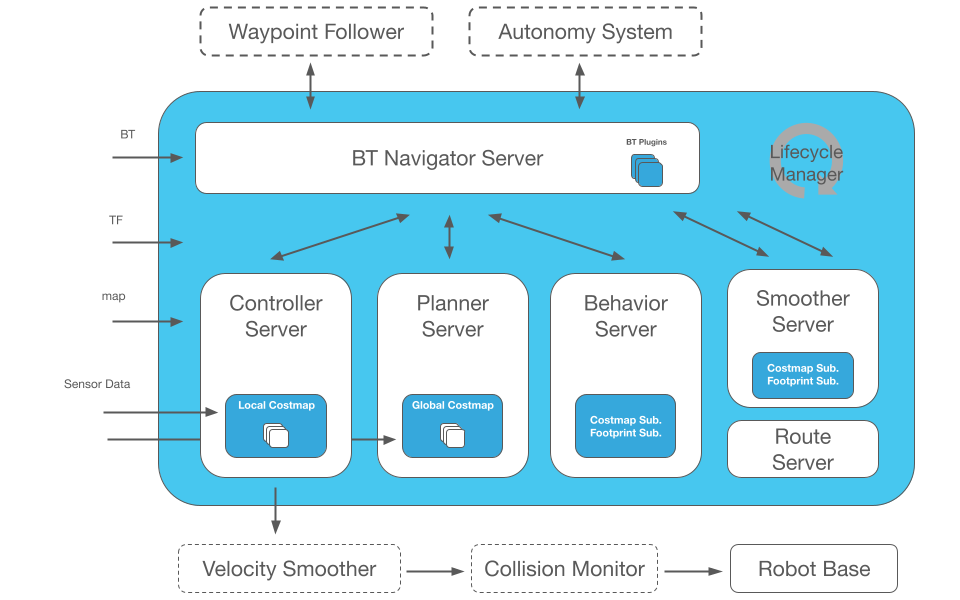
\includegraphics[width=14cm]{nav2_architecture}
}
\caption{Архитектура стэка Nav2}
\end{figure}

В Nav2 есть инструменты для:
\begin{itemize}
	\item загрузки и сохранения карт;
	\item локализации робота по предоставленной карте;
	\item планирования пути через окружающую среду;
	\item управления роботом, чтобы он следовал по маршруту и динамически
		корректировался, чтобы избежать столкновений;
	\item сглаживания маршрутов, чтобы сделать их более плавными;
	\item преобразование данных датчиков в модель окружающего мира;
	\item построение сложных и настраиваемых моделей поведения роботов с
		помощью деревьев поведения;
	\item выполнение заранее определенных действий в случае сбоя, вмешательства
		человека или других ситуаций;
	\item выполнение последовательных маршрутных точек, составляющих миссию;
	\item управление жизненным циклом программы и сторожевым таймером для
		серверов;
	\item мониторинг необработанных данных датчиков на предмет неминуемого
		столкновения или опасной ситуации;
\end{itemize}

\subsection{Анализ пакетов \ros{} решающих задачу одновременной локализации и
картирования}
\label{sec:ros_analysys}

Алгоритмы SLAM можно разделить на две группы: более ранние алгоритмы,
использующие подходы, основанные на фильтрах Байеса, и более новые методы,
основанные на графах. Значимые реализации на основе фильтров, доступные в виде
пакетов \ros{}: GMapping и HectorSLAM. Cartographer и KartoSLAM являются
основными доступными реализациями на основе графов \cite{macenski2021slam}.

Рассмотрим пакеты ros{}, такие как: SLAM Toolbox и GMapping:
\begin{itemize}
	\item SLAM Toolbox -- использует подход оптимизации
		графов.
	\item GMapping \cite{grisetti2005improving} -- использует Rao–Blackwellized
		Particle Filter (Фильтр частиц с использование теоремы Рао -- Блэквелла --
		Колмогорова )
\end{itemize}

% SLAM Toolbox 
% В SLAM Toolbox есть возможность делать почти всё, что есть в любой другой
% платной и бесплатной библиотеке SLAM. Это включает в себя:
В SLAM Toolbox реализованы многие функции которые необходимы для навигации и
постройки карт
\begin{itemize}
	\item точечный 2D SLAM для мобильных роботов, с экспортом карт;
	\item продолжение уточнения карты после остановки, перестройка карты или
		продолжение построения карты из сохраненного файла позиций в любое
		время;
	\item пожизненное картирование -- продолжение построение карты  в течении
		всей работы ПО, одновременно удаляя лишнюю информацию из новых снимков
		лидара.
	\item режим локализации на основе, построенный на основе графа позиций.
		Возможность запуска режима локализации без предварительной карты для
		режима «лидарной одометрии» с локальным замыканием циклов;
	\item синхронный и асинхронный режимы работы;
	\item оптимизационные решатели на основе плагинов с новым оптимизированным
		плагином на основе Google Ceres;
	\item плагин RVIZ для взаимодействия с инструментами;
	\item инструменты манипулирования графами в RVIZ для манипулирования узлами
		и связями графа во время отображения;
	\item сериализация карт и хранение данных без потерь.
\end{itemize}

\begin{figure}[h]
\centering
	\fbox{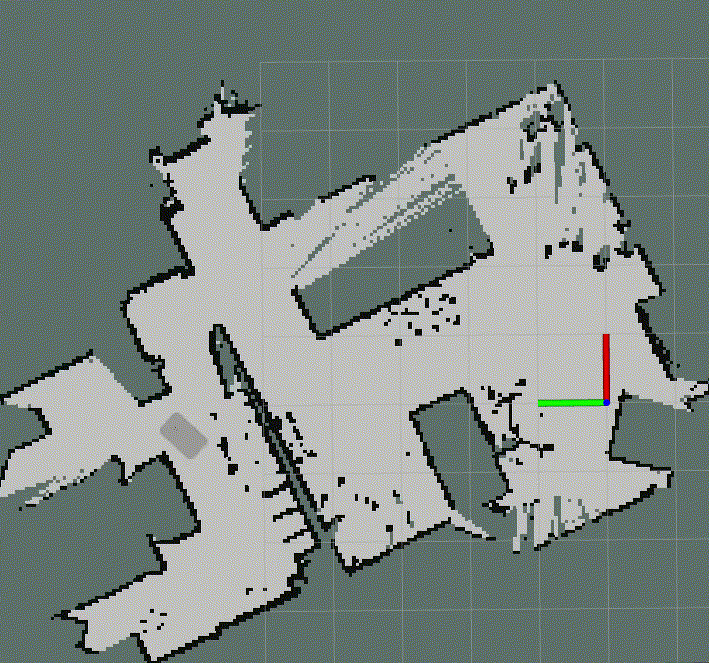
\includegraphics[width=7cm]{slam_toolbox_example}
\centering
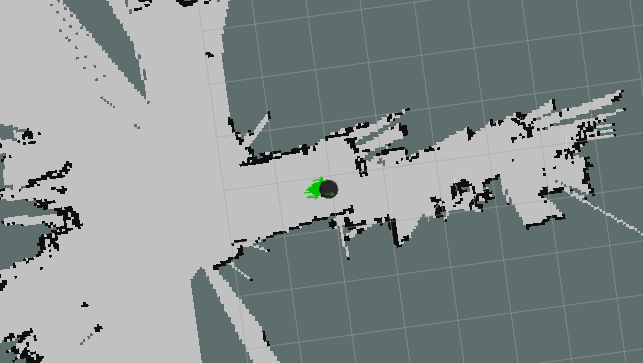
\includegraphics[width=7cm]{gmapping_example}
	}
	\caption{Пример построения карты используя SLAM Toolbox (слева) и GMapping
	(справа).}
	\label{ris:map_example}
\end{figure}

В то время как пакет GMapping предлагает обёртку над алгоритмом,
описанным в статье \cite{grisetti2005improving}, не включая дополнительный
функционал который предоставляется SLAM Toolbox, предоставляя лишь возможность настройки параметров алгоритма и получения построенной карты.




\subsection{Yet Another Robot Platform}
Yet Another Robot Platform (YARP) \cite{metta2006yarp} -- это фреймворк который
преследует цели, очень схожие с \ros{}. YARP поддерживает построение системы
управления роботом как набор программ общающимся в одноранговой сети используя
различные каналы связи, что по своей сути не отличается от целей ros{}. YARP
менее популярен, используется для более специализированных систем и не имеет
отличительных преимуществ, поэтому далее его не рассматриваем.


\subsection{Формирование требований к проектируемому программному средству}

% \todo{Формирование требований}
%
% Исходя из результата анализа существующих аналогов, можно выделить следующие недостатки:

% \begin{itemize}
% 	\item \todo{Недостаток 1}
% \end{itemize}

Исходя из этого, целью дипломного проектирования является разработка
программного средства, способного устранить вышеперечисленные недостатки, а
также реализовать необходимый набор функций характерный для программных средств
в этой области.

Для достижения поставленных целей следует решить следующие задачи: 
\begin{itemize}
	\item определить требования  к  разрабатываемому  программному  средству  и 
	составление спецификации, включающей их; 
	\item осуществить выбор  технологии  и  языка  программирования  для
		реализации программного средства; 
	\item провести проектирование архитектуры программного средства; 
	\item разработка алгоритмов для метода SLAM; 
	\item разработка алгоритмов для оценки местоположения; 
	\item разработка алгоритмов для поиска маршрута; 
	\item разработка алгоритмов для выполнения маршрута; 
	\item программирование и тестирование отдельных программных модулей; 
	\item тестирование готового программного средств.
\end{itemize}

% \todo{Набор функций}

% Для достижения поставленной цели необходимо решить следующие недостатки:
%
% % - Уменьшить потребление памяти
% % - Моментальное обновление карты
% % - Single binary executable
% % - speed of execution
%
% \begin{itemize}
% 	\item \todo{Недостаток}
% \end{itemize}

\section{Моделирование предметной области и разработка функциональных
требований}

\subsection{Сенсоры}

Для получения информации об окружающей среде используются различные сенсоры.

\subsubsection{Lidar}
Сенсор Lidar выдаёт 2D снимок помещения -- облако точек в двумерной плоскости.
Используя облако точек, и зная позицию в которой снимок облака был совершён,
возможно реконструировать карту окружающего пространства на сетке. Если провести
отметить все клетки через которые прошёл луч за пустые, и отметить последнюю
клетку которую луч зацепил в качестве отмеченной, то получается 

\begin{figure}[h]
\centering
	\fbox{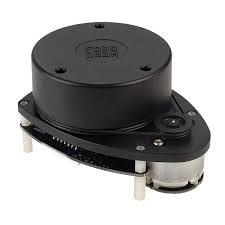
\includegraphics[width=9cm]{2d_lidar}}
\caption{2D Lidar}
\end{figure}

\subsubsection{IMU}
Сенсор IMU выдаёт угловое и линейное ускорение

\subsubsection{GPS}
Сенсор GPS выдаёт глобальную позицию в мировых координатах. Для того чтобы
привести координаты на плоскость используем UTM развёртку для локальной
местности.

\subsection{Общие сведения и требования к работе программного средства}
- Построение карты
- Следование маршруту
- Конфигурация 

\subsection{Описание функциональности программного средства}

\todo{USECASE диаграмма}

\subsection{Спецификация функциональных требований}

- Моделируем навигацию

- Occupancy grid

- Надо переместится в указанную точку на карте
- Способ указывания точки на карте


\todo{ Если цель переместится в указанную точку, для этого надо построить
маршрут, чтобы построить маршрут нужна карта, чтобы построить карту используем
позицию и показания с сенсоров и метод SLAM }

\subsection{Функциональные требования}
    - Функциональные требования
        - Получение данных с датчиков
        - **требования** Спецификация функциональных требования/Разработка
          спецификации фун. треб. + разработка тех. требований

\section{Проектирование программного средства}

\subsection{Разработка архитектуры программного средства}

\todo{Общая схема программы}

\subsection{Разработка архитектуры модуля \todo{MotionEstimation}}

\todo{Схема для motionEstimation}

\subsection{Разработка архитектуры модуля \todo{BigMap}}

\subsection{Разработка архитектуры модуля \todo{ScanMatching}}

\subsection{Разработка архитектуры модуля \todo{TODO}}

\section{Разработка программного средства}

\subsection{Выбор языка разработки}

\todo{Выбрали RUST, потому что он лучшийй!!!}

\subsection{Разработка цикла событий}

\todo{Разработка цикла событий}

\subsection{Разработка модуля \todo{MotionEstimation}}

\subsection{Разработка модуля \todo{BigMap}}

\subsection{Разработка модуля \todo{ScanMatching}}


\section{Тестирование работоспособности программного средства}

\subsection{Тестирование модуля наложения снимков лидара}

\todo{Скриншот из test\_gui про наложение сканов}

\subsection{Тестирование модуля KF}

\todo{Скриншот графиков KF}

\subsection{Интеграционное тестирование в симуляции}

\todo{Робот катается в симуляции}

\subsection{Интеграционное тестирование на роботе}

\todo{Робот катается IRL}

\section{Руководство пользователя}

\subsection{Инструкция по установке RUST}

\subsubsection{Установка на Windows}
	Перейдите на страницу \url{https://www.rust-lang.org/tools/install} и следуйте инструкциям по установке.
    Установщик предложит выбрать одну из опций. Выберите опцию 1, чтобы установить Rust со стандартными настройками.

\subsubsection{Установка на macOS/Linux}
Откройте терминал и выполните следующую команду:

\begin{lstlisting}[language=bash]
curl --proto '=https' --tlsv1.2 -sSf https://sh.rustup.rs | sh
\end{lstlisting}


В процессе установки rustup предложит выбрать один из вариантов. Для стандартной установки выберите опцию 1.

\subsubsection{Проверка установки}
	После установки Rust, закройте и снова откройте терминал, чтобы обновить переменную среды PATH.
	Чтобы проверить, правильно ли установлен Rust, введите следующую команду:
\begin{lstinline}[language=bash]
rustc --version
\end{lstinline}
Вы должны увидеть версию Rust, хэш коммита, дату коммита и дату сборки.


\subsubsection{Установка дополнительных программ}
Необходимо выполнить следующие команды для установки дополнительных зависимостей
в проекте. 

\begin{lstlisting}[language=bash]
    cargo install cross
    cargo install cargo-make
    cargo install sccache
\end{lstlisting}

Их использование позволяет запускать ПС на платформах отличных от
платформы пользователя, ускоряет сборку проекта и позволяет использовать
программы для сборки и запуска проекта.


\subsection{Инструкция по запуску проекта}
С помощью cargo make можно запускать различные команды, список команд приведён ниже.

1 Команда {cross} -- собирает бинарный файл проекта для указанной целевой
архитектуры. Зависит от задачи setup\_features. Использует команду cross с
режимом release, именем бинарного файла проекта, без стандартных функций и с
дополнительными флагами функций на основе FEATURE\_NAME.

2 Команда  {compress\_driver} -- сжимает файлы, связанные с драйверами, для
выбранного ROBO\_MODE. Требует установки ROBO\_MODE и наличия скрипта
compress\_driver.sh. Выполняет скрипт compress\_driver.sh.

3 Команда   {copy\_binary} -- копирует скомпилированный бинарный файл в указанный
путь. Требует установки COPY\_TO\_PATH. Копирует бинарный файл из директории
release целевой архитектуры в указанный путь.

4 Команда    {copy\_config} -- копирует конфигурационные файлы в указанный путь.
Требует установки CONFIG\_FILES и COPY\_TO\_PATH. Перебирает CONFIG\_FILES и
копирует каждый в место назначения.

5 Команда     {copy\_scripts} -- копирует скриптовые файлы в указанный путь. Требует
установки SCRIPT\_FILES и COPY\_TO\_PATH. Копирует каждый скриптовый файл и
выводит BUILD\_FLAGS для отладки.

6 Команда      {rename\_zip} -- переименовывает zip-файлы, добавляя суффикс. Требует
установки SUFFIX. Переименовывает все .zip файлы в текущей директории,
добавляя значение SUFFIX.

7 Команда       {setup\_features} -- настраивает флаги функций для задач, которые их
требуют. Требует установки FEATURE\_NAME. Устанавливает переменную окружения
FEATURE\_FLAG в --features.

8  Команда       {sync\_config} -- получает конфигурационные файлы с удаленного робота.
Требует установки CONFIG\_FILES. Использует scp для копирования
IcpConfig.toml из директории ROBO\_HOME робота в локальную директорию
config/ROBO\_MODE через указанный DEPLOY\_PORT.

9 Команда         {copy\_config\_deploy} -- развертывает конфигурационные файлы на
удаленный робот. Требует установки CONFIG\_FILES. Использует scp для
копирования CONFIG\_FILES в директорию ROBO\_HOME робота.

10 Команда          {run\_oneshot\_script} -- запускает одноразовый скрипт на удаленном
роботе после развертывания. Требует установки ONESHOT\_SCRIPT. Копирует
скрипт на робот, выполняет его через ssh и удаляет после выполнения.

11 Команда           {copy\_binary\_deploy} -- развертывает скомпилированный бинарный файл на удаленный робот. Зависит от copy\_config\_deploy и run\_oneshot\_script.

12            соответствующую systemd-службу, копирует бинарный файл в
ROBO\_HOME и использует указанный DEPLOY\_PORT и SSH-ключ.

13             {scripts\_deploy} -- развертывает файл службы systemd для робота.
Требует наличия файла службы в директории robot\_deployment/ROBO\_MODE.
Копирует файл службы в /etc/systemd/system на роботе, перезагружает демон
systemd, включает и перезапускает службу.

14              {deploy} -- оркестрирует процесс развертывания. Выполняет задачи cross,
copy\_binary\_deploy и scripts\_deploy последовательно для сборки и
развертывания бинарного файла на удаленный робот.

15               {test\_single\_default} -- запускает одиночный тестовый сценарий
параллельно. Зависит от setup\_features и запускает задачу solo\_no\_move в
параллельном режиме с форком.

16                {solo\_no\_move} -- запускает тестовую симуляцию для сценария
solo\_no\_move. Устанавливает переменные окружения SCENARIO\_PATH и
WORK\_DIR и выполняет cargo run --bin test\_sim в директории test\_sim.

17                 {gui} -- запускает тестовый GUI в режиме release. Выполняет cargo run
--release --bin test\_gui в директории tools/test\_gui.

18                  {gui\_debug} -- запускает тестовый GUI в режиме отладки. Выполняет cargo
run --bin test\_gui в директории tools/test\_gui.

19                   {run\_webots\_app} -- запускает приложение Webots. Выполняет команду
webots из директории WEBOTS\_HOME.

20                    {run\_mock\_driver} -- запускает имитацию аппаратного контроллера Webots
в режиме release. Выполняет cargo run --bin
hardware\_mock\_webots\_controller --release в директории
hardware\_mock\_webots\_controller.

21                     {run\_mock\_robot} -- запускает приложение Webots и имитацию драйвера
последовательно. Запускает webots, ждет 5 секунд, затем запускает имитацию
драйвера.

22                      {stop\_mock\_robot} -- останавливает приложение Webots и имитацию
драйвера. Завершает все запущенные процессы webots и
hardware\_mock\_webots\_controller.

23                       {control} -- запускает бинарный файл roboq\_service в режиме release с
функцией eureka. Выполняет cargo run --release --bin roboq\_service
--no-default-features --features eureka.

24                        {brains} -- запускает бинарный файл roboporter в режиме release с
функцией simulation. Устанавливает переменные окружения ICP\_CONFIG и
DEVICE\_CONFIG и выполняет cargo run -bin roboporter -release
-no-default-features -features simulation в директории roboporter.

% \subsection{Управление в tgui}

% \subsection{Интеграция с внешним миром \todo{А надо ли?}}


% CUTOFF
\section{Технико-экономическое обоснование разработки и использования
программного средства навигации мобильных систем}

\subsection{Характеристика программного средства}
Программное средство навигации мобильных систем осуществляет задачу перемещения
и определения местоположения мобильной системы, построение и исполнение 
маршрута с использованием сенсоров и приводов. \appname{} оптимизировано для
навигации голономных колёсных роботов. Предполагается что мобильная система 
управляется через отправку команды установки угловой и линейной скорости. 
Также необходима конфигурация под размеры и движение каждого определённого
робота.

\appname{} выполняет следующие функции:

\begin{itemize}
	\item сбор данных с датчиков;
	\item расчёт текущей позиции;
	\item построение карты;
	\item сохранение и загрузка карты;
	\item планирование маршрута;
	\item планирование движения;
	\item исполнение маршрута, учитывая динамические препятствия.
\end{itemize}


В сравнении с \ros{}, который является наиболее популярным аналогом, \appname{}
упрощает развёртывание, требует меньше вычислительных ресурсов за счёт
минимизации затрат на общении модулей путём расположения их в одном процессе
операционной системы, что позволяет использовать менее мощное аппаратное
обеспечение.

\appname{} получает данные с датчиков, информацию о цели которой ей 
необходимо достигнуть  и отправляет управляющие сигналы на ходовую часть. 
Решается задача локализации, построения маршрута и выполнения маршрута 
к заданной точке. 

\subsection{Расчёты затрат на разработку программного средства}

Расчет затрат на разработку ПО производится в разрезе следующих статей затрат:

\begin{itemize}
	\item затраты на основную заработную плату разработчиков;
	\item затраты на дополнительную заработную плату разработчиков;
	\item отчисления на социальные службы;
	\item прочие затраты (амортизационные отчисления, расходы на 
		электроэнергию, командировочные расходы, арендная плата за офисные
		помещения и оборудование, расходы на управление и реализацию и т. п.).
\end{itemize}

Расчёт основной заработной платы осуществляется по формуле

\begin{equation}
	\label{eq:зарплата}
	\text{З}_o = \text{К}_{\text{пр}}\sum_{i=0}^{n} \text{З}_{\text{ч}i} \cdot t_i
	\ \text{,}
\end{equation}


\begin{explanationx}
	\item[где]  $n$  -- категории исполнителей, занятых разработкой
		программного средства;
	\item $\text{К}_\text{пр}$ - коэффициент премий и иных стимулирующих
		выплат (\num{1.3});
	\item $\text{З}_\text{ч}$ --  Часовой оклад исполнителя $i\text{-й}$
		категории, р.;
	\item $t$  -- трудоёмкость работ, выполняемых исполнителем $i\text{-й}$
		категории, ч.
\end{explanationx}


Затраты на основную заработную плату команды разработчиков
делятся исходя из численности, состава команды (категорий исполнителей), 
размеров месячной заработной платы каждого из участников команды, а также
общей трудоёмкости разработки ПО. 

\def \hoursPerMonth {167}

Согласно постановлению Министерства труда и социальной защиты Республики
Беларусь от 15 ноября 2024 г. \No 67 «Об установлении расчетной нормы рабочего
времени на 2024 год» при полной норме продолжительности рабочего времени на
2025 год для пятидневной рабочей недели с выходными днями в субботу и
воскресенье расчетная норма рабочего времени составит \num{2007} ч. На основании
этих данных среднее количество рабочих ч. в месяце принято равным
\hoursPerMonth{} ч.

Трудоёмкость определялась на основе сложности разработки программного средства,
объема функций. За основу в том числе брались фактические значения трудоёмкости
работ при разработке ПО со схожим функционалом в месте прохождения 
преддипломной практики.

Для расчёта возьмём размер премии 20\%.

На основании плановых данных был выполнен расчет основной заработной платы
команды разработчиков, результаты которого приведены в таблице~\ref{table:initialCost}.

\def \devSalary {2700}
\def \devAmountOfHours {458}
\FPeval{\devHourlySalary}{round(\devSalary / \hoursPerMonth, 2)}
\FPeval{\devCost}{round(\devAmountOfHours * \devHourlySalary, 2)}

\def \testSalary {2100}
\def \testAmountOfHours {200}
\FPeval{\testHourlySalary}{round(\testSalary / \hoursPerMonth, 2)}
\FPeval{\testCost}{round(\testAmountOfHours * \testHourlySalary, 2)}

\def \managerSalary {2500}
\def \managerAmountOfHours {120}
\FPeval{\managerHourlySalary}{round(\managerSalary / \hoursPerMonth, 2)}
\FPeval{\managerCost}{round(\managerAmountOfHours * \managerHourlySalary, 2)}

\FPeval{\costSum}{round(\devCost + \testCost + \managerCost, 2)}
\FPeval{\costBonuses}{round(\costSum * 0.2, 2)}
\FPeval{\costTotal}{round(\costSum + \costBonuses, 2)}

%\FloatBarrier
%\bgroup
%\def\arraystretch{1.7}
\nohyphens{
	\begin{longtable}{@{\extracolsep{\fill}}| p{3.5cm} | p{3.5cm} | l | l | l | r |@{}}
		\caption{Расчёт основной заработной платы команды разработчиков}
		\label{table:initialCost} \\
		\hline 
		Наименование должности разработчика
		& Вид выполненной работы
		%& \raisebox{-2cm}{\rotatedtext{\parbox{3.5cm}
		%	{\centering Вид выполненной работы}}}
		& \raisebox{-2cm}{\rotatedtext{\parbox{3.5cm}
			{\centering Месячная заработная плата, р.}}}
		& \raisebox{-2cm}{\rotatedtext{\parbox{3.5cm}
			{\centering Часовая заработная плата, р.}}}
		& \raisebox{-2cm}{\rotatedtext{\parbox{3.5cm}
			{\centering Трудоёмкость работ, ч}}}
		& \raisebox{-2cm}{\rotatedtext{\parbox{3.5cm}
			{\centering Сумма, р.}}}
		\\ \hline 
		\endfirsthead

		Руководитель проекта
		& Координация работы, контроль сроков и этапов разработки
		& \num{\managerSalary}
		& \num{\managerHourlySalary}
		& \num{\managerAmountOfHours}
		& \num{\managerCost}
		\\ \hline 

		Инженер-программист 
		& Разработка программного средства  
		& \num{\devSalary}
		& \num{\devHourlySalary}
		& \num{\devAmountOfHours}
		& \num{\devCost}
		\\ \hline 

		Специалист по тестированию программного обеспечения
		& Тестирование программного средства
		& \num{\testSalary}
		& \num{\testHourlySalary}
		& \num{\testAmountOfHours}
		& \num{\testCost}
		\\ \hline 

		\multicolumn{5}{|l|}{Итого}
		& \num{\costSum}
		\\ \hline

		\multicolumn{5}{|l|}{Премия (20\%)}
		& \num{\costBonuses}
		\\ \hline

		\multicolumn{5}{|l|}{Общая сумма затрат на разработку}
		& \num{\costTotal}
		\\ \hline
	\end{longtable}
}
%\end{table}
%\egroup
%\FloatBarrier

Расчёт затрат на дополнительную заработную плату команды разработчиков.

Затраты на дополнительную заработную плату команды разработчиков включают
выплаты, предусмотренные законодательство о труде (оплата трудовых отпусков,
льготных ч., времени выполнения государственных обязанностей и других выплат,
не связанных с основной деятельностью исполнителей), и определяются по формуле

\begin{equation}
	\text{З}_\text{д} = \frac{\text{З}_\text{о} \cdot
	\text{Н}_\text{д}}{\num{100}}
	\ \text{,}
\end{equation}

\begin{explanationx}
	\item[где] $\text{З}_\text{о}$ -- затраты на основную заработную плату;
	\item $\text{Н}_\text{д}$ -- норматив дополнительной заработной платы
		(\num{15}\%).
\end{explanationx}

Дополнительная заработная плата составит

\FPeval{\additionalSalary}{round(\costTotal * 0.15, 2)}

\begin{equation}
	\text{З}_\text{о} = \frac{\num{\costTotal} \cdot \num{15}}{\num{100}} =
	\num{\additionalSalary}
	\ \text{р.}
\end{equation}


Отчисления на социальные нужды определяются по формуле

\begin{equation}
	\text{Р}_\text{соц} = \frac{(\text{З}_\text{о} + \text{З}_\text{д}) \cdot
	\text{Н}_\text{соц}}{\num{100}}
	\ \text{,}
\end{equation}

\begin{explanationx}
	\item[где] $\text{Н}_\text{соц}$ -- норматив отчислений от фонда оплаты
		труда (35\%).
\end{explanationx}

Отчисления на социальные нужды составят

\FPeval{\socialCost}{round((\costTotal + \additionalSalary) * 0.35, 2)}
\begin{equation}
	\text{Р}_\text{соц} = \frac{(\num{\costTotal} + \num{\additionalSalary}) \cdot
	\num{35}}{\num{100}} = \num{\socialCost}
	\ \text{р.}
\end{equation}

Прочие затраты рассчитываются по формуле

\begin{equation}
	\text{Р}_\text{пз} = \frac{\text{З}_\text{о} \cdot \text{Н}_\text{пз}}{\num{100}}
	\ \text{,}
\end{equation}

\begin{explanationx}
\item[где] $\text{Н}_\text{пз}$ -- норматив прочих затрат, 35\%.
\end{explanationx}

Прочие затраты составят

\FPeval{\etcCost}{round(\costTotal * 0.35, 2)}
\begin{equation}
	\text{Р}_\text{пз} = \frac{\num{\costTotal} \cdot \num{35}}{\num{100}} = \num{\etcCost}
	\ \text{р.}
\end{equation}

Общая сумма затрат на разработку рассчитывается по формуле
\begin{equation}
	\text{З}_\text{общ} = 
	\text{З}_\text{о} +
	\text{З}_\text{д} +
	\text{Р}_\text{соц} +
	\text{Р}_\text{пз}
	\ \text{.}
\end{equation}

\FPeval{\finalCost}{round(\costTotal + \additionalSalary + \socialCost +
\etcCost, 2)}

Расчёт затрат на разработку программного продукта предоставлен в таблице~\ref{table:totalCost}

\FloatBarrier
\begin{table}
	\caption{Затраты на разработку программного обеспечения}
	\label{table:totalCost}
	\begin{tabular}{|l|r|}
		\hline
		Наименование статьи затрат
		& Значение, р.
		\\ \hline

		1. Основная заработная плата разработчиков
		& \num{\costTotal}
		\\ \hline

		2. Дополнительная заработная плата разработчиков
		& \num{\additionalSalary}
		\\ \hline

		3. Отчисления на социальные нужды
		& \num{\socialCost}
		\\ \hline

		4. Прочие затраты
		& \num{\etcCost}
		\\ \hline

		Общая сумма инвестиций в разработку
		& \num{\finalCost}
		\\ \hline
	\end{tabular}
\end{table}
\FloatBarrier

\subsection{Экономический эффект от разработки программного обеспечения и
применения программного обеспечения для собственных нужд}

В общем виде экономический эффект при использовании ПО рассчитывается по формуле
по формуле
\begin{equation}
	\Delta\text{П}_\text{ч} = (\text{Э}_\text{з} - \text{И}_\text{разр} -\Delta\text{З}_\text{тек})
	\cdot (1 - \frac{\text{Н}_\text{п}}{\num{100}})
	\ \text{,}
\end{equation}

\def \nalogNaPribil{20}

\begin{explanationx}
	\item[где] $\text{Э}_\text{з}$ -- экономия текущих затрат, полученная в
		результате применения ПО, р.;
	\item $\text{И}_\text{разр}$ -- затраты на разработку программного
		обеспечения, р.
	\item $\Delta\text{З}_\text{тек}$ -- прирост текущих затрат, связанных с
		поддержкой и сопровождением ПО, р.;
	\item $\text{Н}_\text{п}$ -- ставка налога на прибыль согласно действующему
	законодательству (\nalogNaPribil\%).
\end{explanationx}

% Дополнительная стоимость для сопровождения, в процентах
\def \additionalSupportCost {10}
\FPeval{\supportCost}{round(\finalCost * \additionalSupportCost / 100, 2)}
Прирост текущих затрат, связанных с сопровождением и поддержкой ПО, примем за
\num{\additionalSupportCost}\% от затрат на разработку ПО, что составит
\begin{equation}
	\text{З}_\text{тек} = \num{\finalCost} \cdot
	\frac{\num{\additionalSupportCost}}{\num{100}} = \num{\supportCost}
	\ \text{р.}
\end{equation}

% TODO, использование заменить на применение, но это уже было согласовано и абобус

Использование данного программного средства позволяет использовать более дешёвое
аппаратное обеспечение. Так как навигация и SLAM являются ресурсоёмкими
операциями, обычно используют компьютер \linebreak{}
NVIDIA~Jetson~Nano, стоимостью \num{1421.83} р.,
в то время как \appname{} позволяет использовать
Banana~Pi~CM4, стоимостью \num{300.12} р.

\FPeval{\savingsResult}{round(1421.83 - 300.12, 2)}
\def \robotCount {40}
\FPeval{\costWin}{round(\robotCount * \savingsResult, 2)}

Это позволяет экономить \num{\savingsResult} р. на единицу продукции.
Если взять в расчёт что в год производится  \num{\robotCount} мобильных систем,
получаем экономию текущих затрат в \num{\costWin} р.

\FPeval{\totalWin}{round((\costWin - \supportCost - \finalCost) * (1 -
0.\nalogNaPribil), 2)}

Экономический эффект для организации-заказчика при использовании ПО и выпуске
партии в \num{\robotCount} единиц составляет
\begin{equation}
	\Delta\text{П}_\text{ч} = (\num{\costWin} - \num{\finalCost} - \num{\supportCost}) \cdot
	(\num{1} - \frac{\num{\nalogNaPribil}}{\num{100}}) = \num{\totalWin}
	\ \text{р.}
\end{equation}

Уровень рентабельность затрат рассчитывается по формуле
\begin{equation}
	\text{У}_\text{р} = \frac{\Delta\text{П}_\text{ч}}{\text{И}_\text{разр}}
\cdot \num{100}
	\ \text{,}
\end{equation}

уровень рентабельности составляет

\FPeval{\rentabelnost}{round(\totalWin / \finalCost * 100, 2)}
\begin{equation}
	\text{У}_\text{р} = \frac{\num{\totalWin}}{\num{\finalCost}} \cdot \num{100}
	= \num{\rentabelnost}\%
	\ \text{.}
\end{equation}


\def \stavkaBankov {0.1376}


В результате расчёта были получены следующие показатели (см.~табл.~
\bgroup
\def\arraystretch{1.2}
\ref{table:hehelastone})
	\begin{longtable}{|p{10cm}|c|}
		\caption{Экономические показатели} 
		\setlength{\belowcaptionskip}{0pt}
		\setlength{\abovecaptionskip}{0pt}
		\label{table:hehelastone} \\
		\hline
		Наименование показателя
		& Значение
		\\ \hline

		Прогнозируемая сумма затрат на разработку программного продукта
		& \num{\finalCost}~р.
		\\ \hline

		Прирост чистой прибыли
		& \num{\totalWin}~р.
		\\ \hline

		Рентабельность инвестиций
		& \num{\rentabelnost}\%
		\\ \hline
	\end{longtable}
\egroup



Средняя процентная ставка по банковским депозитным вкладам на январь
2025-го г. не превышает \num{13.76}\% \cite{nbrb2025}, рентабельность инвестиций
в проект составляет \num{\rentabelnost}\%. Инвестиции в разработку проекта
окупятся за первый год реализации проекта. Это означает, что данный проект
программного средства навигации мобильных систем является экономический
эффективным, разработка и последующая продажа программного продукта являются
экономически целесообразными.


\sectioncentered*{Заключение}
\label{sec:ending}
\addcontentsline{toc}{section}{\nameref{sec:ending}}
% \todo{REWORK THIS ACCORDING TO OTHER DIPLOMAS}

В ходе выполнения дипломного проекта было разработано программное средство на
языке программирования Rust для навигации мобильных систем. Основной задачей
разработки было создание эффективного и минималистичного инструмента для
построения карт и обеспечения навигации при минимизации зависимостей от
сторонних библиотек и операционных систем, что повышает переносимость и
надежность решения.

В рамках реализации программного обеспечения были успешно реализованы следующие
ключевые функциональные модули:

\begin{itemize}
	\item алгоритмы совмещения сканов, включающие в себя методы Iterative
		Closest Point (ICP), Corellative Scan Matcher (CSM) и Multi-Scale
		Corellative Scan Matcher (MSCM), обеспечивающие точное и надежное
		создание локальных карт на основе данных сенсоров;
	\item алгоритмы глобальной навигации, позволяющие планировать маршруты и
		обеспечивать ориентацию мобильной платформы в пространстве с учетом
		глобальной карты;
	\item алгоритмы локальной навигации, направленные на обеспечение
		безопасного и эффективного движения робота в непосредственной близости
		от препятствий и динамических объектов.
\end{itemize}


В процессе работы был проведен комплексный анализ предметной области,
включающий обзор и критический анализ существующих решений и технологий в
области навигации мобильных роботов. Это позволило выявить
основные недостатки и ограничения существующих библиотек и определить
направления для оптимизации.

Результаты работы подтвердили достижение всех поставленных целей и задач
дипломного проекта. Полученное программное средство демонстрирует высокую
производительность, надежность и гибкость, что делает его перспективным
инструментом для применения в различных робототехнических системах.

В качестве направлений дальнейшего развития проекта рассматривается оптимизация
программного кода с целью повышения производительности и снижения
ресурсопотребления, а также расширение функциональности за счет внедрения
дополнительных алгоритмов совмещения сканов и навигации.

Таким образом, завершенный проект вносит значительный вклад в область
разработки программного обеспечения для робототехники и открывает новые
возможности для создания высокоэффективных и надежных автономных навигационных
систем.


\renewcommand{\bibsection}{\sectioncentered*{Список использованных источников}\label{sec:literat}}
\addcontentsline{toc}{section}{\nameref{sec:literat}}
\bibliography{test}

\sectioncentered*{Приложение А}
\vspace{-\baselineskip + 5pt}
\begin{center}
	\bfseries\normalsize
	(обязательное) \\
Текст программного средства 
\end{center}

\addcontentsline{toc}{section}{Приложение А (обязательное) Текст программного средства}

\lstset{breaklines=true, breakatwhitespace=false,
  alsoletter={.},
}
\lstinputlisting[breaklines=true]{dump2}

\end{document}
